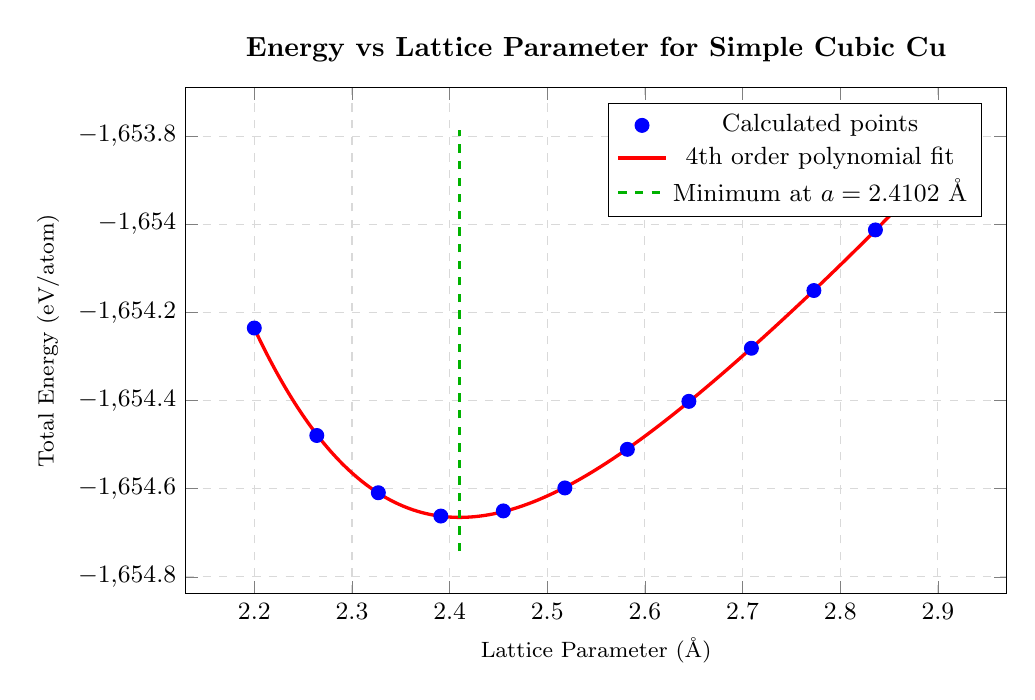
\begin{tikzpicture}
\begin{axis}[
    width=12cm,
    height=8cm,
    xlabel={Lattice Parameter (\AA)},
    ylabel={Total Energy (eV/atom)},
    title={Energy vs Lattice Parameter for Simple Cubic Cu},
    grid=major,
    grid style={dashed, gray!30},
    legend pos=north east,
    legend style={font=\small},
    tick label style={font=\small},
    label style={font=\footnotesize},
    title style={font=\bfseries}
]

% Calculated points
\addplot[
    only marks,
    mark=*,
    mark size=2.5pt,
    color=blue,
] coordinates {
    (2.200000, -1654.235499)
    (2.264000, -1654.479341)
    (2.327000, -1654.609246)
    (2.391000, -1654.662157)
    (2.455000, -1654.650467)
    (2.518000, -1654.598390)
    (2.582000, -1654.510761)
    (2.645000, -1654.401865)
    (2.709000, -1654.281368)
    (2.773000, -1654.150380)
    (2.836000, -1654.012876)
    (2.900000, -1653.865733)
};
\addlegendentry{Calculated points}

% Polynomial fit
\addplot[
    color=red,
    line width=1.2pt,
    smooth,
] coordinates {
    (2.200000, -1654.236377)
    (2.207007, -1654.268728)
    (2.214014, -1654.299521)
    (2.221021, -1654.328794)
    (2.228028, -1654.356582)
    (2.235035, -1654.382921)
    (2.242042, -1654.407846)
    (2.249049, -1654.431392)
    (2.256056, -1654.453593)
    (2.263063, -1654.474482)
    (2.270070, -1654.494094)
    (2.277778, -1654.514230)
    (2.284785, -1654.531264)
    (2.291792, -1654.547121)
    (2.298799, -1654.561832)
    (2.305806, -1654.575427)
    (2.312813, -1654.587938)
    (2.319820, -1654.599393)
    (2.326827, -1654.609824)
    (2.333834, -1654.619258)
    (2.340841, -1654.627725)
    (2.347848, -1654.635253)
    (2.355556, -1654.642482)
    (2.362563, -1654.648128)
    (2.369570, -1654.652918)
    (2.376577, -1654.656880)
    (2.383584, -1654.660039)
    (2.390591, -1654.662422)
    (2.397598, -1654.664052)
    (2.404605, -1654.664954)
    (2.411612, -1654.665152)
    (2.418619, -1654.664670)
    (2.425626, -1654.663530)
    (2.433333, -1654.661545)
    (2.440340, -1654.659098)
    (2.447347, -1654.656063)
    (2.454354, -1654.652461)
    (2.461361, -1654.648312)
    (2.468368, -1654.643636)
    (2.475375, -1654.638454)
    (2.482382, -1654.632784)
    (2.489389, -1654.626647)
    (2.496396, -1654.620059)
    (2.503403, -1654.613039)
    (2.511111, -1654.604840)
    (2.518118, -1654.596969)
    (2.525125, -1654.588720)
    (2.532132, -1654.580107)
    (2.539139, -1654.571147)
    (2.546146, -1654.561855)
    (2.553153, -1654.552245)
    (2.560160, -1654.542331)
    (2.567167, -1654.532128)
    (2.574174, -1654.521649)
    (2.581181, -1654.510907)
    (2.588889, -1654.498800)
    (2.595896, -1654.487544)
    (2.602903, -1654.476062)
    (2.609910, -1654.464364)
    (2.616917, -1654.452461)
    (2.623924, -1654.440363)
    (2.630931, -1654.428080)
    (2.637938, -1654.415621)
    (2.644945, -1654.402994)
    (2.651952, -1654.390207)
    (2.658959, -1654.377270)
    (2.666667, -1654.362872)
    (2.673674, -1654.349639)
    (2.680681, -1654.336275)
    (2.687688, -1654.322787)
    (2.694695, -1654.309180)
    (2.701702, -1654.295458)
    (2.708709, -1654.281627)
    (2.715716, -1654.267690)
    (2.722723, -1654.253650)
    (2.729730, -1654.239512)
    (2.736737, -1654.225277)
    (2.744444, -1654.209510)
    (2.751451, -1654.195079)
    (2.758458, -1654.180557)
    (2.765465, -1654.165944)
    (2.772472, -1654.151241)
    (2.779479, -1654.136448)
    (2.786486, -1654.121564)
    (2.793493, -1654.106588)
    (2.800501, -1654.091518)
    (2.807508, -1654.076352)
    (2.814515, -1654.061089)
    (2.822222, -1654.044182)
    (2.829229, -1654.028703)
    (2.836236, -1654.013114)
    (2.843243, -1653.997413)
    (2.850250, -1653.981594)
    (2.857257, -1653.965652)
    (2.864264, -1653.949580)
    (2.871271, -1653.933374)
    (2.878278, -1653.917026)
    (2.885285, -1653.900529)
    (2.892292, -1653.883876)
    (2.900000, -1653.865367)
};
\addlegendentry{4th order polynomial fit}

% Vertical line at minimum
\addplot[
    color=green!70!black,
    dashed,
    line width=1pt,
] coordinates {
    (2.410210, -1654.741800)
    (2.410210, -1653.786091)
};
\addlegendentry{Minimum at $a=2.4102$ \AA}

\end{axis}
\end{tikzpicture}